\section{Linear Time Series Analysis}
\paragraph{Primary Text Reading.} \citeA[chap. 2]{tsay2005aft}\index{Tsay, Ruey}

A collection of asset returns, such as the log returns of an asset \eqref{eq:log-return} is a \emph{linear time series}. Some of the elements of this analysis are: stationarity, dynamic dependence, autocorrelation function, modeling, and, forecasting. Models include:
\begin{enumerate}
\item simple autoregressive (AR)
\item simple moving average (MA)
\item mixed autoregressive moving-average (ARMA)
\item seasonal models
\item unit-root nonstationary
\item regression models with time series errors
%\item fractionally differenced models for long-range dependence
\end{enumerate}

\subsection{Stationarity}
Strict stationarity occurs when joint distributions $P(X \cap Y)$ are time-invariant, or in other words, $X:(r_{t_1}, \ldots, r_{t_k})$ is identical to $Y:(r_{t_{1+t}}, \ldots, r_{t_{k+t}})$ for all $t$. A weak stationarity exists if the mean of $r_t$ and the covariance between $r_t$ and $r_{t-\ell}$ are time-invariant, where $\ell$ is an arbitrary integer. What this means in practice is that asset values fluctuate with constant variation around a fixed level so that we can make inferences about future observations. The mean, or expectation, of returns is therefore $\mu = E(r_t)$ and the variance of returns is $\text{Var}(r_t) = E[(r_t - \mu)^2]$.

\subsection{Correlation and ACF}
The correlation coefficient between two random variables $X$ and $Y$ is
\[
\boxed{\quad \rho_{X,Y}={\mathrm{cov}(X,Y) \over \sigma_X \sigma_Y} ={E((X-\mu_X)(Y-\mu_Y)) \over \sigma_X\sigma_Y}, \quad}
\]
where $\mu_X$ and $\mu_Y$ are expected values of $X$ and $Y$ respectively, and $\sigma_X$ and $\sigma_Y$ are its standard deviations. Thus, the sample correlation is
\begin{eqnarray}
r_{xy}&=&\frac{\sum x_iy_i-n \bar{x} \bar{y}}{(n-1) s_x s_y} \\
\smallskip
&=&\frac{n\sum x_iy_i-\sum x_i\sum y_i} {\sqrt{n\sum x_i^2-(\sum x_i)^2}~\sqrt{n\sum y_i^2-(\sum y_i)^2}}. \notag
\end{eqnarray}

\paragraph{Autocorrelation Function (ACF).} When we want to examine the linear dependence between $r_t$ and its previous values $r_{t-\ell}$ we are interested in the lag-$\ell$ \emph{autocorrelation} of the series $r_t$.
\marginpar{\begin{small}\begin{flushleft}\textcolor{blue}{Existence of serial correlations implies that the return is predictable, indicating market inefficiency.}\end{flushleft}\end{small}}
The extent to which the series exhibits autocorrelation can help us determine how much of today's asset value has been determined by previous values. We could perform a hypothesis test for zero serial correlations, which would imply market efficiency,
\begin{eqnarray*}
H_0 : r_{XY} &=& 0 \\
H_a : r_{XY} &\ne& 0.
\end{eqnarray*}
Our null hypothesis $H_0$ is that this market is efficient, and our alternative hypothesis $H_a$ is that this market is \emph{not} efficient. Some sources of serial correlations found in \fts{} are,
\begin{itemize}
\item Nonsynchronous trading (Section~\ref{High-Frequency}) 
\item Bid-ask bounce (Section~\ref{High-Frequency}) 
\item Risk premium, \textit{etc}. (Section~\ref{Conditional Heteroskedastic})
\end{itemize}
Thus, significant sample ACF does not necessarily imply market 
inefficiency. 

\paragraph{Portmanteau test.} To look for autocorrelation, we will run a \emph{portmanteau test}\index{Portmanteau test}, which tests whether any of a group of autocorrelations of a time series are different from zero. Two portmanteau tests we will use are the Box-Pierce test and the Ljung-Box test. The Ljung-Box test can be defined as \\
$H_0$: 	The data are random. \\
$H_a$: 	The data are not random.
\bigskip

The Ljung-Box test statistic is calculated as
\begin{equation}
Q_{LB}=n(n+2)\sum_{k=1}^s r_k^2/(n-k).
\label{eq:Ljung-Box}
\end{equation}
where, \\
$n$ = number of observations \\
$s$ = number of coefficients to test autocorrelation \\
$r_k$ = autocorrelation coefficient (for lag $k$).
\bigskip

If the sample value of $Q_{LB}$ exceeds the critical value of a chi-square distribution with $s$ degrees of freedom, then at least one value of $r$ is statistically different from zero at the specified significance level. The null hypothesis is that none of the autocorrelation coefficients up to lag $s$ is different from zero.

We will use R to examine autocorrelation graphically, and then to perform a test for randomness, or lack of serial correlation of data.
\begin{verbatim}
rets<-read.table("aapl.txt")
s1<-acf(rets$Log.Return, lag=15, main="Autocorrelation of AAPL")
s1$acf
Box.test(rets, lag=15)
Box.test(rets, lag=15, type="Ljung")
\end{verbatim}

The dotted lines in Figure~\ref{figure:aapl-acf} represent the 95\% confidence interval of the ACF function. Notice that the vertical lines do not cross the dotted line boundary, which would indicate statistical significance from zero.

The first \texttt{Box.test} gives us the \emph{Box-Pierce test}\index{Box-Pierce test} of our log returns with $\chi$-squared = 14.7735, df = 15, $p$-value = 0.4679. The second \texttt{Box.test} gives us the \emph{Ljung-Box test}\index{Ljung-Box test}, $\chi$-squared = 15.0983, df = 15, $p$-value = 0.4444.

\begin{figure}[tb]
  \centering
  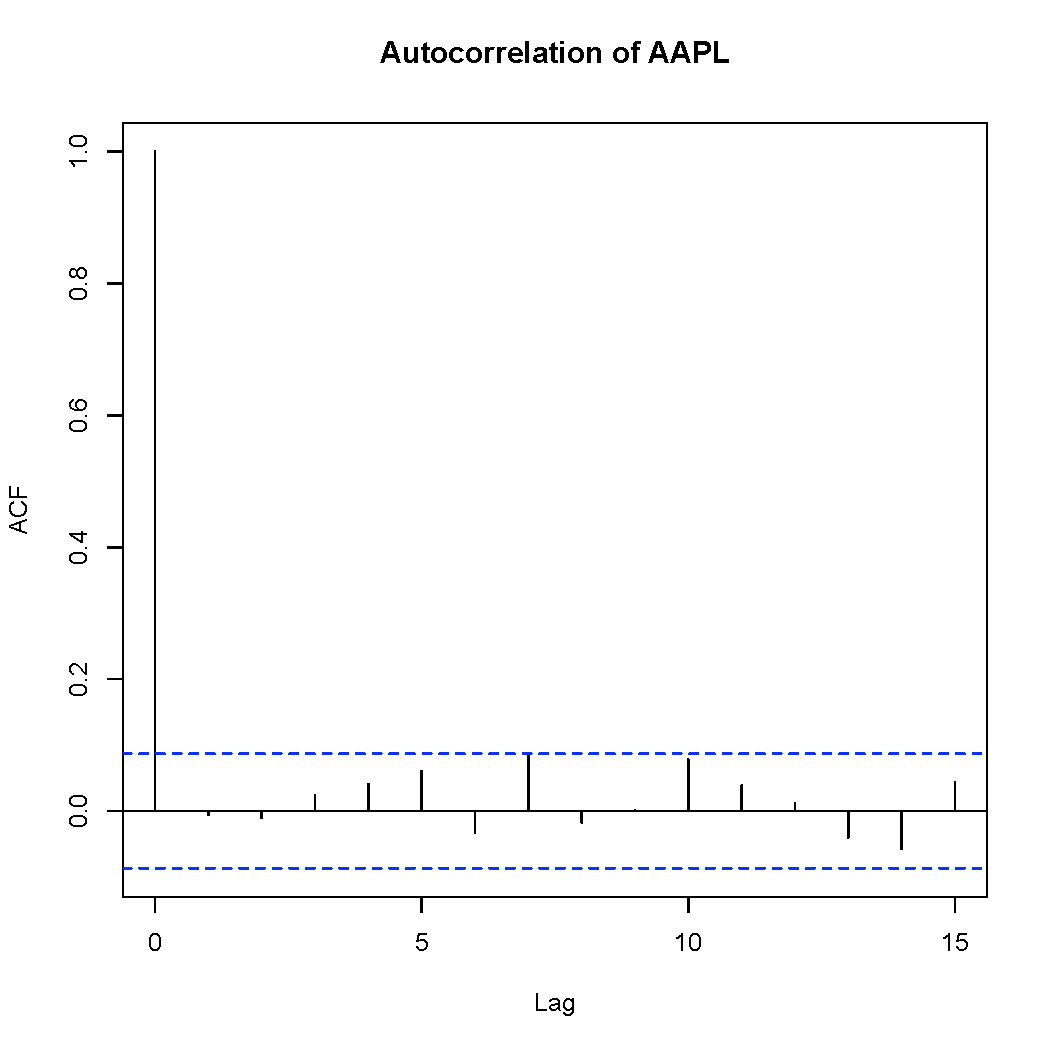
\includegraphics[scale=.6]{aapl-acf}
  \caption{ACF function of AAPL log returns with 15-day lag.}
  \label{figure:aapl-acf}
\end{figure}

Using R to generate the appropriate $\chi$-squared statistic to determine the critical region, \texttt{qchisq(p=0.4444, df=15)}, we get 13.60595. The hypothesis of randomness is rejected if $Q_{LB} > \chi^2(p, df)$. In this case, since our $p$-value is not more extreme than our $\alpha$ of 0.05, we do not reject the hypothesis that the data are random.

\pagebreak
\begin{figure}[tb]
  \centering
  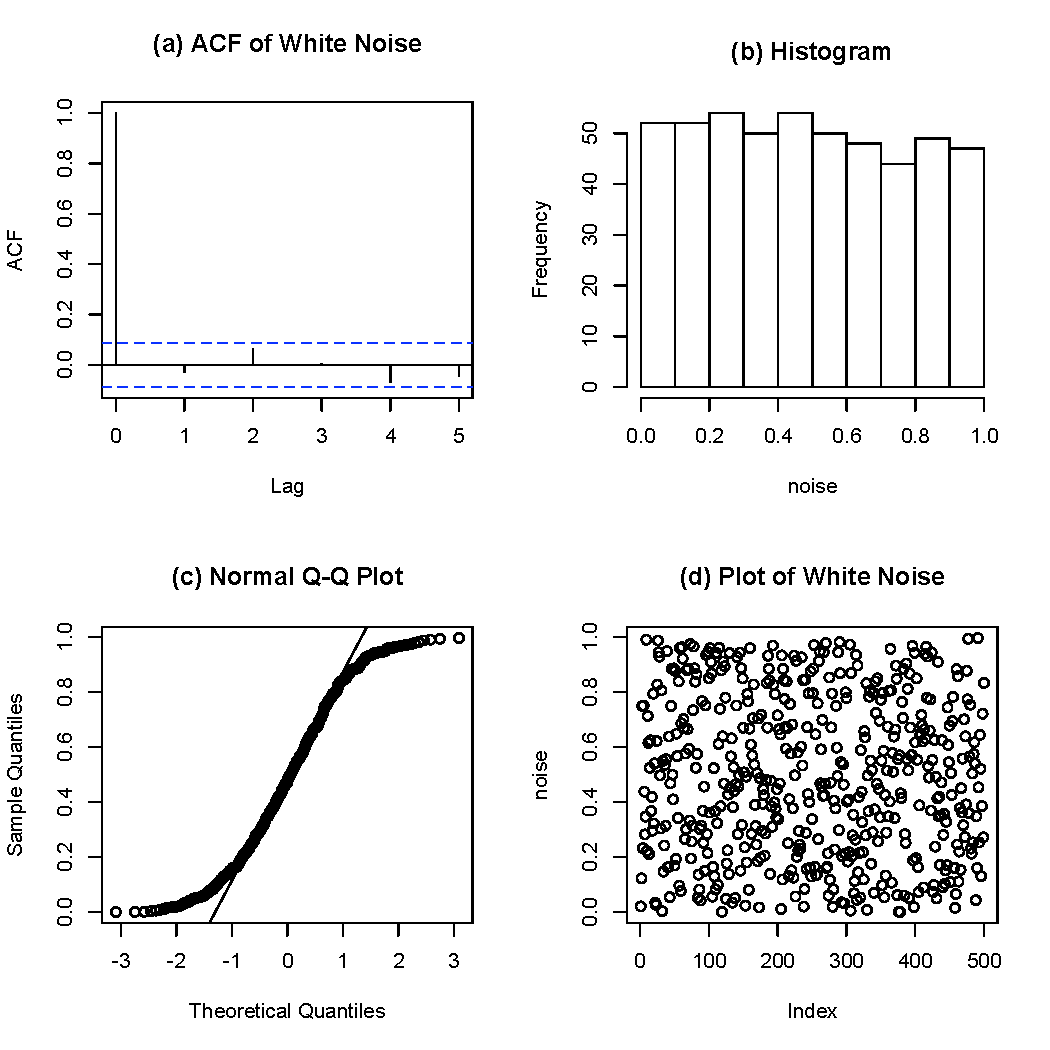
\includegraphics[scale=.7]{noise}
  \caption[Properties of White Noise]{White noise has an ACF of zero as seen in (a). We see in (b) a nearly uniform distribution, and in (c) we observe that the tails are not normally distributed. The values are plotted in (d).}
  \label{figure:noise}
\end{figure}

\paragraph{White Noise.}\index{White Noise}\index{Time Series!white noise} A time series $r_t$ that is a sequence of iid random variables with a finite mean and variance is \emph{white noise}. The serial correlation of any two points in $r_t$, regardless of lag, is zero, thus ACF values of white noise is zero. Using R to demonstrate, we can see the results in Figure~\ref{figure:noise}. In some circumstances, log returns of asset values can be considered white noise. With this assumption, we can create linear time series models.
\ecaption{White Noise in R}
\begin{verbatim}
noise=runif(5000) # Random numbers from Uniform Distribution
layout(rbind(c(1,2), c(3,4)))
acf(noise,lag=5, main="(a) ACF of White Noise")
hist(noise, main="(b) Histogram")
qqnorm(noise, main="(c) Normal Q-Q Plot")
qqline(noise)
plot(noise, main="(d) Plot of White Noise")
\end{verbatim}

Thus, we can implement a linear time series as
\begin{equation}
r_t = \mu + \sum^{\infty}_{i=0} \psi_i a_{t-i}
\end{equation}
where $\mu$ is the mean of $r_t$, $\psi_0=1$, and $\{a_t\}$ is a sequence of iid random variables.

\subsection{Simple Autoregressive Models}
Within a linear time series, there may exist a certain random movement, described as white noise $a_t$ with a mean of zero and variance of $\sigma^2_a$. This allows us to create a simple model
\begin{equation}
r_t = \phi_0 +\phi_1 r_{t-1} + a_t,
\label{eq:ar1}
\end{equation}
which follows the form of simple linear regression, where $r_t$ is the dependent variable, and $r_{t-1}$ is the independent variable. Equation~\eqref{eq:ar1} is the autoregressive (AR) model of order 1, also known as AR(1). We can generalize \eqref{eq:ar1} to the AR($p$) model
\begin{equation}
r_t = \phi_0 +\phi_1 r_{t-1} + \cdots + \phi_p r_{t-p} + a_t.
\label{eq:arp}
\end{equation}

\paragraph{AR Models.} We assume that \eqref{eq:ar1} has weak stationarity, and $E(r_t)=\mu$, $\text{Var}(r_t)=\gamma_0$, and $\text{Cov}(r_t,r_{t-j})=\gamma_j$, where $\mu$ and $\gamma_0$ are constant and $\gamma_j$ is a function of $j$, not $t$. This gives us a weakly stationary AR(1) model
\[
\text{Var}(r_t) = \gamma_0=\frac{\sigma^2}{1-\phi^2_1}, \text{ and \:} \gamma_{\ell}=\phi_1\gamma_{\ell-1}, \text{ for \:} \ell>0
\]
using the results of
\[
\gamma_{\ell} =
	\begin{cases}
	\phi_1 \gamma_1 + \sigma^2_a & \text{if $\ell=0$,} \\
	\phi_1 \gamma_{\ell-1} & \text{if $\ell>0$,}
	\end{cases}
\]
where we use $\gamma_{\ell}=\gamma_{-\ell}$. 

\subsubsection{Partial Autocorrelation Function (PACF)}\index{Partial Autocorrelation Function\\ (PACF)}
Before working with an AR($p$) time series, it is necessary to find out what $p$ represents. This process is called \emph{order determination} of an AR model, and we work our out in terms of order $p$,

\begin{eqnarray*}
r_t &=& \phi_{0,1} + \phi_{1,1} r_{t-1} + e_{1t}, \\
r_t &=& \phi_{0,2} + \phi_{1,2} r_{t-1} + \phi_{2,2} r_{t-2} + e_{2t}, \\
r_t &=& \phi_{0,3} + \phi_{1,3} r_{t-1} + \phi_{2,3} r_{t-2} + \phi_{3,3} r_{t-3} + e_{3t}, \\
\vdots && \vdots \\
r_t &=& \phi_{0,n} + \phi_{1,n} r_{t-1} + \phi_{n+1,n+2} r_{t-1-n} + \cdots + e_{nt}.
\end{eqnarray*}

These models are solved as multiple linear regressions with the lag period increasing with each equation. Thus, we can see the added contribution of each lag coefficient. We compare ACF and PACF in Figure~\ref{figure:pacf}.

\begin{figure}[tb]
  \centering
  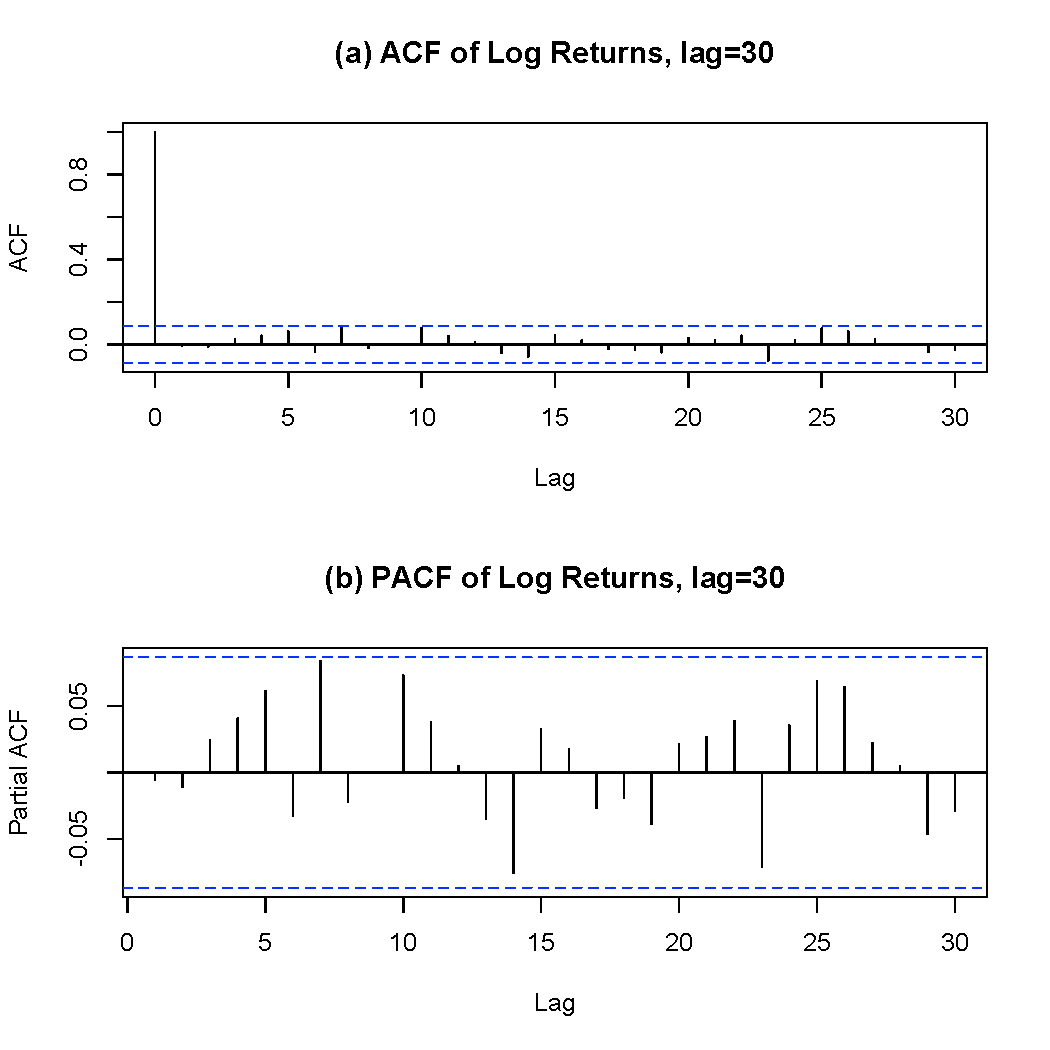
\includegraphics[scale=.6]{pacf}
  \caption[Comparing ACF with PACF]{(a) ACF function of AAPL log returns with 30-day lag. (b) PACF function of AAPL log returns with 30-day lag.}
  \label{figure:pacf}
\end{figure}

\subsubsection{Information Criterion Function}
Another way to determine the order $p$ of an AR process is by using a likelihood function such as the \emph{Akaike information criterion (AIC)}\index{Akaike information criterion (AIC)}, which measures goodness of fit of a model, and penalizes excessive use of parameters $k$.
\begin{equation}
AIC=\frac{-2}{n} \ln(\text{likelihood}) + \frac{2}{n} \times k,
\end{equation}
where the likelihood function is evaluated at the maximum likelihood estimates, \\
$n$ = sample size, \\
$k$ =  number of parameters.

\subsubsection{Goodness of Fit}
A conventional statistic to measure goodness of fit of a stationary model is $r^2$,
\begin{equation}
r^2 = 1 - \frac{\sum^T_{t=p+1}\hat{a}^2_t}{\sum^T_{t=p+1}(r_t-\bar{r})^2}
\end{equation}
where $\bar{r}= \left( \sum{T}{t=p+1} r_t\right) / (T-p)$. Yet, this only applies to a stationary time series. As a replacement, the \emph{adjusted $r^2$} is offered,
\begin{eqnarray*}
\text{Adj $r^2$} &=& 1 - \frac{\text{Variance of residuals}}{\text{Variance of $r_t$}} \\
&=& 1- \frac{\hat{\sigma}^2_a}{\hat{\sigma}^2_r}.
\end{eqnarray*}


\subsubsection{Forecasting}
Much of the purpose of \fts{} is forecasting. The AR($p$) model in \eqref{eq:arp} can be used to model a forecast. If we at time index $h$ and we forecast $r_{h+\ell}$, where $\ell \ge 1$, then $h$ is our \emph{forecast origin}\index{Forecast origin} and $\ell$ is our \emph{forecast horizon}\index{Forecast horizon}. Let $\hat{r}_h(\ell)$ be the forecast of $r_{h+\ell}$ using the minimum squared error loss function and $F_h$ is the collection of information at the forecast origin $h$. Then, the forecast $\hat{r}_k(\ell)$ is chosen such that
\[
E\{[r_{h+\ell} - \hat{r}_h(\ell)]^2 | F_h \} \le \min_g E[(r_{h+\ell}-g)^2 | F_h],
\]
where $g$ is a function of he information available at time $h$ (inclusive), that is, a function of $F_h$. We referred to $\hat{r}_h$ as the $\ell$-step ahead forecast of $r_t$, at the forecast origin $h$.

\margincomment[red]{The $\phi$ parameters are to be estimated from the data.}
\paragraph{1-Step Ahead Forecast.} Using \eqref{eq:arp}, we see
\[
r_{h+1} = \phi_0 + \phi_1 r_h + \cdots + \phi_p r_{h+1-p} + a_{h+1}.
\]
Under the minimum squared error loss function, the point forecast of $r_{h+1}$ given that $F_h=\{r_h, r_{h-1}, \ldots \}$ is the conditional expectation
\[
\hat{r}_h(1)=E(r_{h+1} | F_h) = \phi_0 + \sum^{p}_{i=1} \phi_i r_{h+1-i},
\]
and the associated forecast error is
\[
e_h(1)=r_{h+1} - \hat{r}_h(1) = a_{h+1}.
\]
The process can be extended to 2-step ahead and beyond by simple extension. The conditional expectation and forecast error are also adjusted accordingly.

\paragraph{Multistep Ahead Forecast.} A generalization of 1-step ahead forecast is an $\ell$-step ahead forecast
\begin{equation}
\hat{r}_h(\ell) = \phi_0 + \sum^{p}_{i=1} \phi_i \hat{r}_h(\ell-i),
\label{eq:multistep-forecast}
\end{equation}
where $\hat{r}_h(i)=r_{h+i}$ if $i \le 0$. This forecast can be computed recursively using forecasts $\hat{r}_h(i)$ for $i= \{1, \ldots, \ell-1 \}$. The $\ell$-step ahead forecast error is $e_h(\ell)=r_{h+\ell}-\hat{r}_h(\ell)$. It can be shown that for a stationary AR($p$) model, $\hat{r}_h(\ell)$ converges to $E(r_t)$ as $\ell \rightarrow \infty$, meaning that for such a series long-term point forecast approaches its unconditional mean. This property is \emph{mean reversion}\index{Mean reversion}, and appears in literature, notably in interest rate studies.

In an AR(1) model, the speed of mean reversion is measured by the \emph{half-life} defined as $k=\ln(0.5 / \left| \phi_1 \right| )$, which is defined as the number of periods required for the magnitude of the forecast to become one-half of the forecast origin. The variance of the forecast error approaches the unconditional variance of $r_t$.

We see in Figure~\ref{figure:gnp-acf} a plot of 176 observations of U.S. GNP changes. In panel (a), it appears that although the changes fluctuate, they tend to return to a central point indicated by the red dashed line, a point of mean reversion. The lag is changed from lag-1 to lag-2, and we observe a slight upward drift, which is consistent with our seeing that panel (a) has a mean slightly greater than zero (0.007741, actually). Next, we look for the presence of autocorrelation. The R code to examine GNP changes and ACF is very simple.

\ecaption{Examining GNP Changes and ACF function in R}
\begin{verbatim}
gnpdata=read.table("q-gnp4791.txt")
GNP=gnpdata[,1]
par(mfcol=c(2,2)) # put 4 plots on one page
plot(GNP,type="l",main="(a)") 
abline(mean(GNP),0, col="red",lty=4)
plot(GNP[1:175], GNP[2:176], main="(c)")
plot(GNP[1:174], GNP[3:176], main="(b)")
acf(GNP, lag=12, main="(d)") 

\end{verbatim}

\begin{figure}[tb]
  \centering
  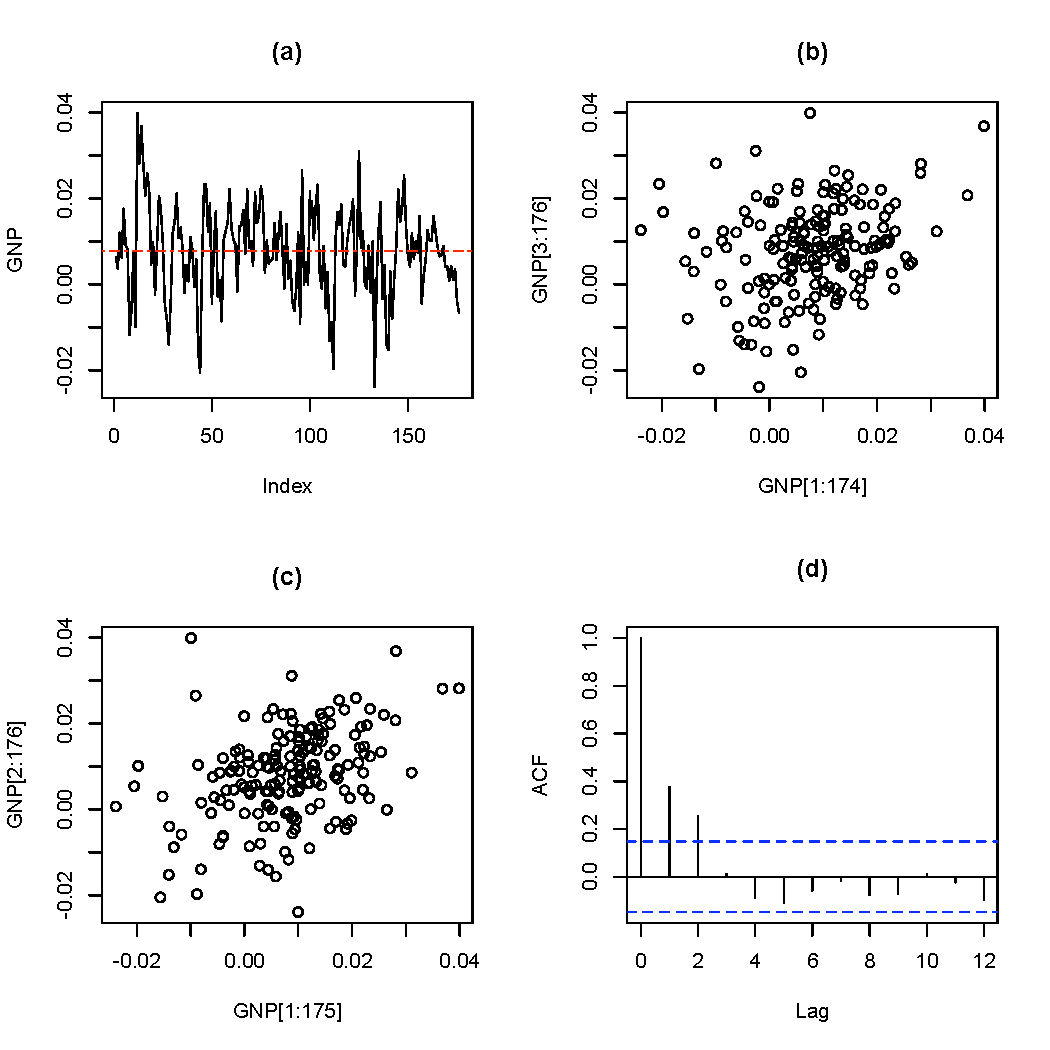
\includegraphics[scale=.65]{gnp-acf}
  \caption[Analysis of U.S. GNP with ACF function]{After plotting changes in U.S. GNP (a), we compare lag-1 (b), to lag-2 (c), and then see that the 12-period ACF function (d) finds autocorrelation at lag-1 and lag-2.}
  \label{figure:gnp-acf}
\end{figure}

\subsection{Simple Moving-Average Models}\index{Simple Moving-Average Models}
Another type of \fts{} model is the \emph{moving average} (MA) model. Initially, an MA model is understood as an AR model of infinite order
\[
r_t = \phi_0 + \phi_1 r_{t-1} + \cdots + \phi_{\infty} r_{\infty}.
\]
This is unrealistic because we have an infinite number of parameters. We will replace it with an MA($\ell$) model of finite order, specifically, $\ell$
\[
X_t = \varepsilon_t + \sum_{i=1}^\ell \theta_i \varepsilon_{t-i}.
\]

\paragraph{MA Models.} MA models are always weakly stationary because they are finite linear combinations of a white noise sequence for which the first two moments are time-invariant. To discover the order of an MA model, we may use an ACF function. We see from Figure~\ref{figure:pacf} what the 30-day lag looks like with AAPL log returns. Using that lag, we plot the log returns, its mean, and a 30-day moving average is superimposed in blue in Figure~\ref{figure:aapl-ret-ma30}.

\begin{figure}[tb]
  \centering
  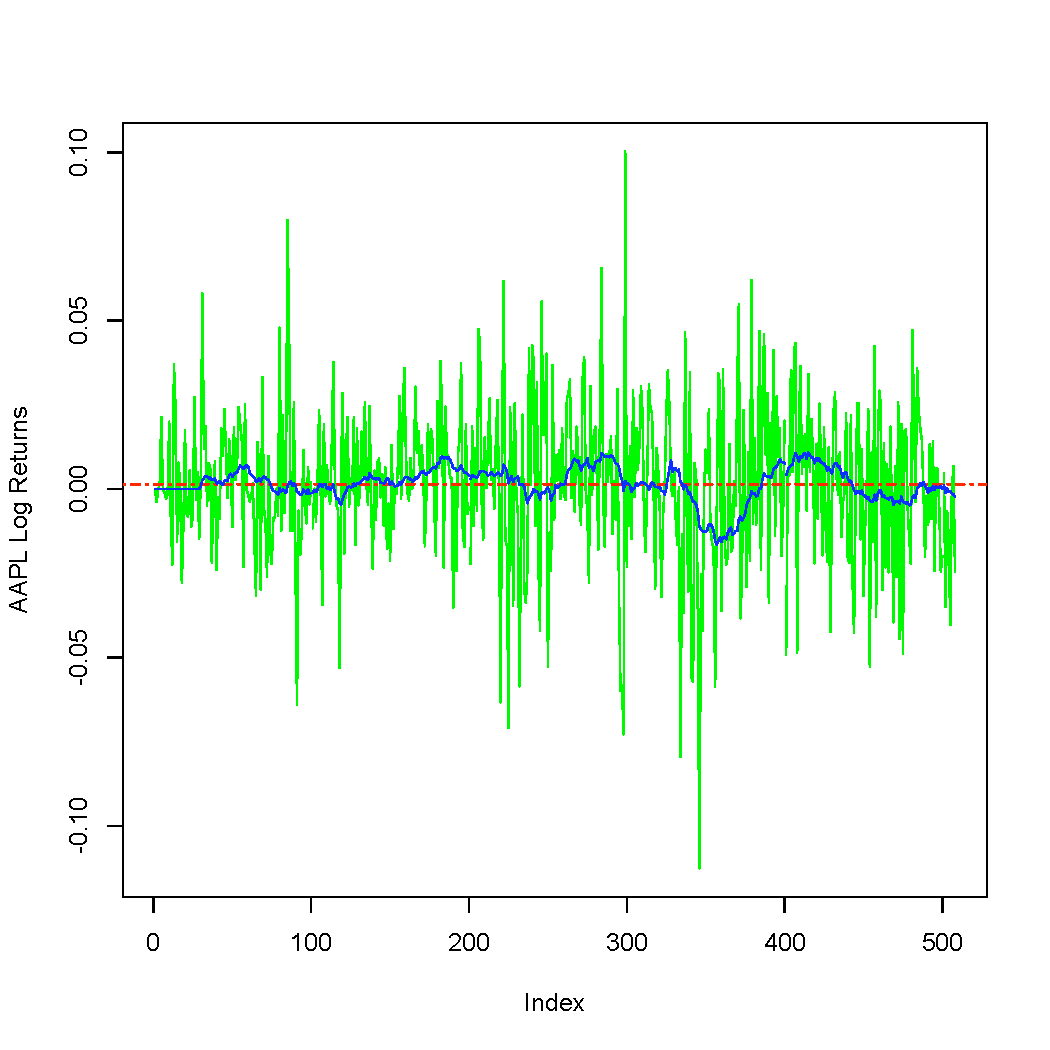
\includegraphics[scale=.6]{aapl-ret-ma30}
  \caption[AAPL Log Returns and MA(30)]{AAPL log return plotted in green. The mean plotted in red and dashed line. The 30-day moving average is superimposed in blue.}
  \label{figure:aapl-ret-ma30}
\end{figure}


\pagebreak
\subsection{Simple ARMA Models}\index{ARMA Models}
\margincomment{ARMA models are used with volatility modeling more than with returns series.}
Having briefly discussed both AR and MA models, we discover that a model of multiple order may be required to perform adequate modeling and forecasting. A remedy for this is the autoregressive moving-average (ARMA) model, which is a combined model that keeps the number of parameters small. It is also important to understand ARMA models as a building block to GARCH models, which are discussed in Section~\ref{garch}.

A time series $r_t$ follows an ARMA(1,1) model if it satisfies
\begin{equation}
r_t - \phi_1 r_{t-1} = \phi_0 + a_t - \theta_0 + a_t - \theta_1 a_{t-1},
\label{eq:arma1-1}
\end{equation}
where $\{a_t\}$ is a white noise series. The left-hand side of \eqref{eq:arma1-1} is the AR component and the right-hand side is the MA component. The constant term is $\phi_0$. To avoid cancellation of both sides, which would make \eqref{eq:arma1-1} a white noise series, we require that $\phi_1 \ne \theta_1$.

\paragraph{ARMA(1,1) Models.} Since ARMA(1,1) models are generalizations of AR(1) models with modifications to allow inclusion of a MA(1) component, we already know much about these models, such as the stationarity condition is the same. There is a notable differences, the ACF of an ARMA(1,1) model looks like a AR(1) model except that the exponential decay starts with lag 2 instead of lag 1. The general form of an ARMA($p,q$) model is
\[
r_t = \phi_0 + \sum^p_{i=1} \phi_i r_{t-1} + a_t - \sum^q_{i=1} \theta_i a_{t-i},
\]
where $\{a_t\}$ is a white noise series and $p$ and $q$ are non-negative integers.

Using ACF and PACF are not very useful in determining the order of an ARMA model. \citeA{tsaytiao1984eacf} propose an alternative approach, which is known as the \emph{extended autocorrelation function} (EACF).\index{Extended Autocorrelation Function \\(EACF)} This function is used to specify the order of an ARMA process. The aim is to derive the MA component from a consistent estimate of the AR component of an ARMA model.

\paragraph{Forecasting with ARMA.} A 1-step ahead forecast $r_{h+1}$ of an ARMA model is
\[
\hat{r}_h(1)=E(r_{h+1}|F_h)=\phi_0 + \sum^p_{i=1} \phi_i r_{h+1-i} - \sum^q_{i=1} \theta_i a_{h+1-i},
\]
where $h$ is the forecast origin, and $F_h$ is the available information.

\subsection{Unit-Root Nonstationarity}\index{Unit-Root Nonstationarity}
Several types of \fts{} are nonstationary, such as interest rates, foreign exchange currency rates, and asset price series because they have no fixed level of price. This condition is all referred to as \emph{unit-root nonsationarity}.  The best known example of this is a random-walk model.

A random walk is a time series $\{p_t\}$ that satisfies the condition
\begin{equation}
p_t = p_{t-1}+a_t,
\label{eq:random-walk}
\end{equation}
where $p_0$ is the starting value and $\{a_t\}$ is white noise.

Using a simple R statement, \texttt{plot(cumsum(rnorm(20000)),type="l")} used three times, we create three random walks that seem to converge in Figure~\ref{figure:three-walks}. One obvious problem is that the price time series drops below zero on several occasions. A nominal price or rate will never be below zero, but a \emph{real rate}, one compared to another over time, may become negative.
\begin{figure}[tb]
  \centering
  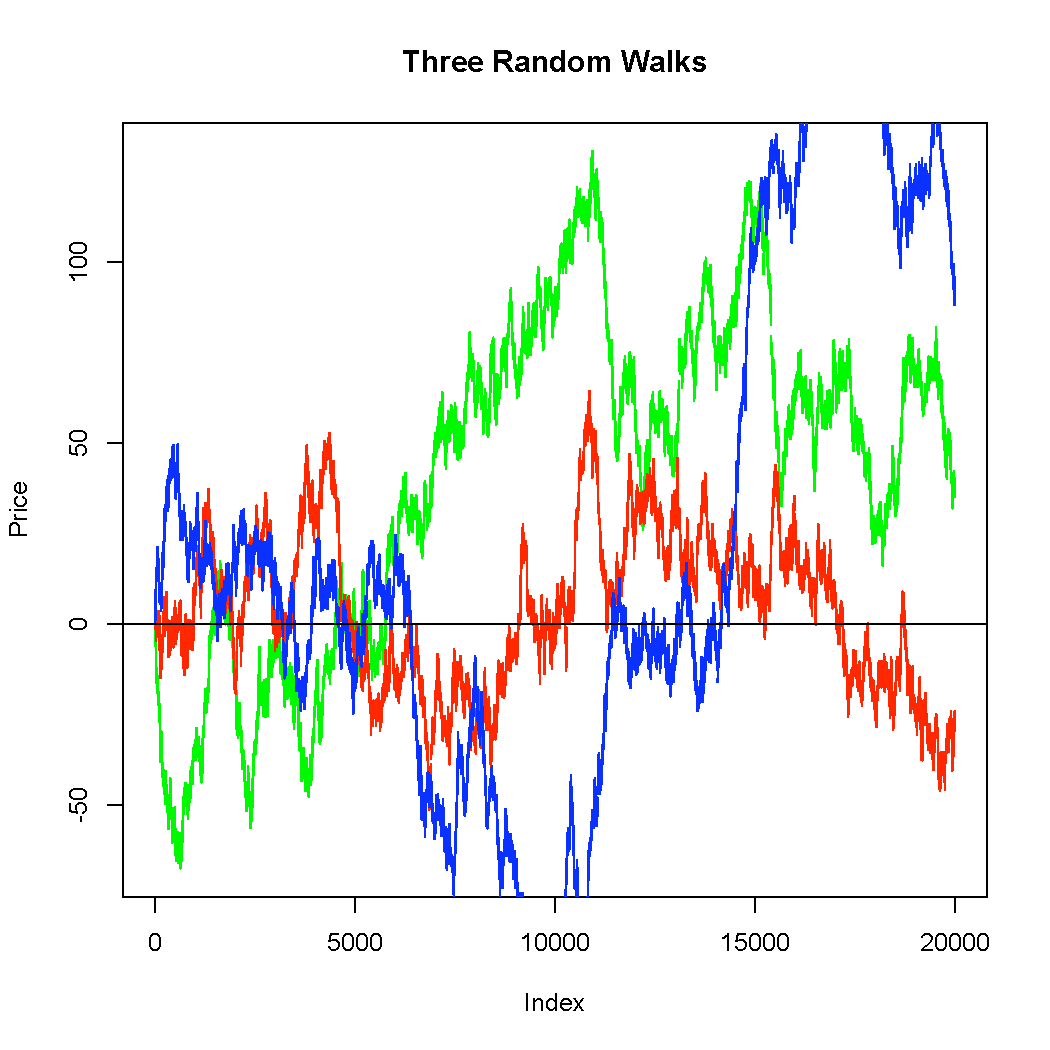
\includegraphics[scale=.6]{three-walks}
  \caption[Three Random Walks, no Drift]{Three random walks, with no drift, yet they seem to converge.}
  \label{figure:three-walks}
\end{figure}

If we treat \eqref{eq:random-walk} as a kind of AR(1) model, then the coefficient of $p_{t-1}$ is one (\emph{or unity}), which does not satisfy the weak stationarity condition of an AR(1) model. Therefore, a random-walk series is a unit-root nonstationary time series.  This kind of series is not predictable or mean-reverting.

The MA representation of \eqref{eq:random-walk} is
\[
p_t = a_t + a_{t-1} + a_{t-2} + \cdots,
\]
which may continue indefinitely. The $\ell$-step ahead forecast error is
\[
e_h(\ell) = a_{h+\ell} + \cdots + a_{h+1},
\]
which means that $\text{Var}[e_h(\ell)] = \ell \sigma^2$, and it diverges to infinity as $\ell \to \infty$. Again, this model is not predictable because the usefulness of the point forecast $\hat{p}_h(\ell)$ diminishes as $\ell$ increases.

\paragraph{Random Walk with Drift.} Observing markets, it becomes clear that the log return series exhibits a positive mean, which would indicate some form of drift.
\begin{equation}
p_t = \mu +p_{t-1} + a_t,
\end{equation}
where $\mu=E(p_t - p_{t-1})$ and $\{a_t\}$ is white noise. The $\mu$ term is vital to the model because it represents the time trend of the log price $p_t$, and is referred to as the \emph{drift}.

\subsubsection{Trend-Stationary Time Series}
A model that is related to random walk with drift is the trend-stationary time series model
\[
p_t = \beta_0 + \beta_1 t+r_t
\]
where $r_t$ is a stationary time series, such as a stationary AR($p$) series. We observe that $p_t$ grows in time on a linear scale $\beta_1$.

\subsubsection{Unit-Root Nonstationary Models}
Modifying an ARMA model by allowing the AR polynomial to have 1 as a characteristic root, the model becomes the autoregressive integrated moving-average (ARIMA)\index{Autoregressive Integrated\\ Moving-Average (ARIMA)} model. A common way to handle unit-root nonstationarity is by \emph{differencing}\index{Differencing}.

\paragraph{Differencing.} Price time series are seen as nonstationary, but log returns are stationary. A way to transform a non-stationary model into a stationary one is by \emph{differencing}. The first difference series of $y_t$ is
\[
c_t = y_t - y_{t-1}.
\]
Also, if $s_t$ follows an ARMA($p,q$) model, then $y_t$ is an ARIMA($p,2,q$) process.

\paragraph{Unit-Root Test.}\index{Unit-root test} To test whether a log price series $p_t$ follows random walk or random walk with drift, we use
\begin{subequations}
	\begin{eqnarray}
	p_t &=& \phi_1 p_{t-1} + e_t, \label{eq:unit-root-a} \\
	 &=& \phi_0 + \phi_1 p_{t-1} + e_t \label{eq:unit-root-b}
	\end{eqnarray}
\end{subequations}
where $e_t$ is an error term comprising white noise, and we may using either \eqref{eq:unit-root-a} or \eqref{eq:unit-root-b} to examine the unit testing problem, which is set up as the \emph{Dickey-Fuller Test.}\index{Dickey-Fuller Test}\\
\begin{eqnarray*}
H_0: \phi_1 = 1 \\
H_a: \phi_1 < 1
\end{eqnarray*}
The test statistic is a $t$-ratio of least square estimate of $\phi_1$. For instance, the least square method for \eqref{eq:unit-root-a} is
\[
\hat{\phi}_1 = \frac{\sum^T_{t=1}p_{t-1}p_t}{\sum^T_{t=1}p^2_{t-1}}, \qquad
\hat{\sigma}^2_e = \frac{\sum^T_{t=1}(p_t-\hat{\phi}_1 p_{t-1})^2}{T-1},
\]
where $p_0=0$ and $T$ is the sample size. The Dickey-Fuller test $t$-ratio is
\[
DF \equiv \text{$t$-ratio} = \frac{\hat{\phi}_1-1}{\text{std}(\hat{\phi}_1)} 
= \frac{\sum^T_{t=1}p_{t-1}e_t}{\hat{\sigma}_e \sqrt{\sum^T_{t=1}p^2_{t-1}}}
\]

When modeling economic time series, it is better to use ARIMA($p,d,q$) than the simpler \eqref{eq:unit-root-b}, although AR($p$) models are also often used.

\paragraph{Testing ARIMA Models.} The three components $(p, d, q)$ of ARIMA are the AR order $p$, the degree of differencing $d$, and the MA order $q$. Using the R functions \texttt{arima} and \texttt{AIC} we will test several combinations of an ARIMA($p,d,q$) model and get an AIC value for each. The smaller the AIC, the better the model fits the data.

\ecaption{Testing ARIMA Models in R}
\begin{verbatim}
# Test AR order p by itself: ARIMA(p,0,0)
model100<-arima(aapl$Close,order=c(1,0,0))
model200<-arima(aapl$Close,order=c(2,0,0))
AIC(model100, model200)

# Test the MA order q by itself: ARIMA(0,0,q)
model001<-arima(aapl$Close,order=c(0,0,1))
model002<-arima(aapl$Close,order=c(0,0,2))
AIC(model001,model002)

# Now hold AR constant, change MA
model100<-arima(aapl$Close,order=c(1,0,0))
model101<-arima(aapl$Close,order=c(1,0,1))
model102<-arima(aapl$Close,order=c(1,0,2))
AIC(model100,model101,model102)

# Test the degree of differencing d
model100<-arima(aapl$Close,order=c(1,0,0))
model110<-arima(aapl$Close,order=c(1,1,0))
AIC(model100,model110)
\end{verbatim}

\subsection{Seasonal Models}\index{Seasonal Models}
\begin{figure}[tb]
  \centering
  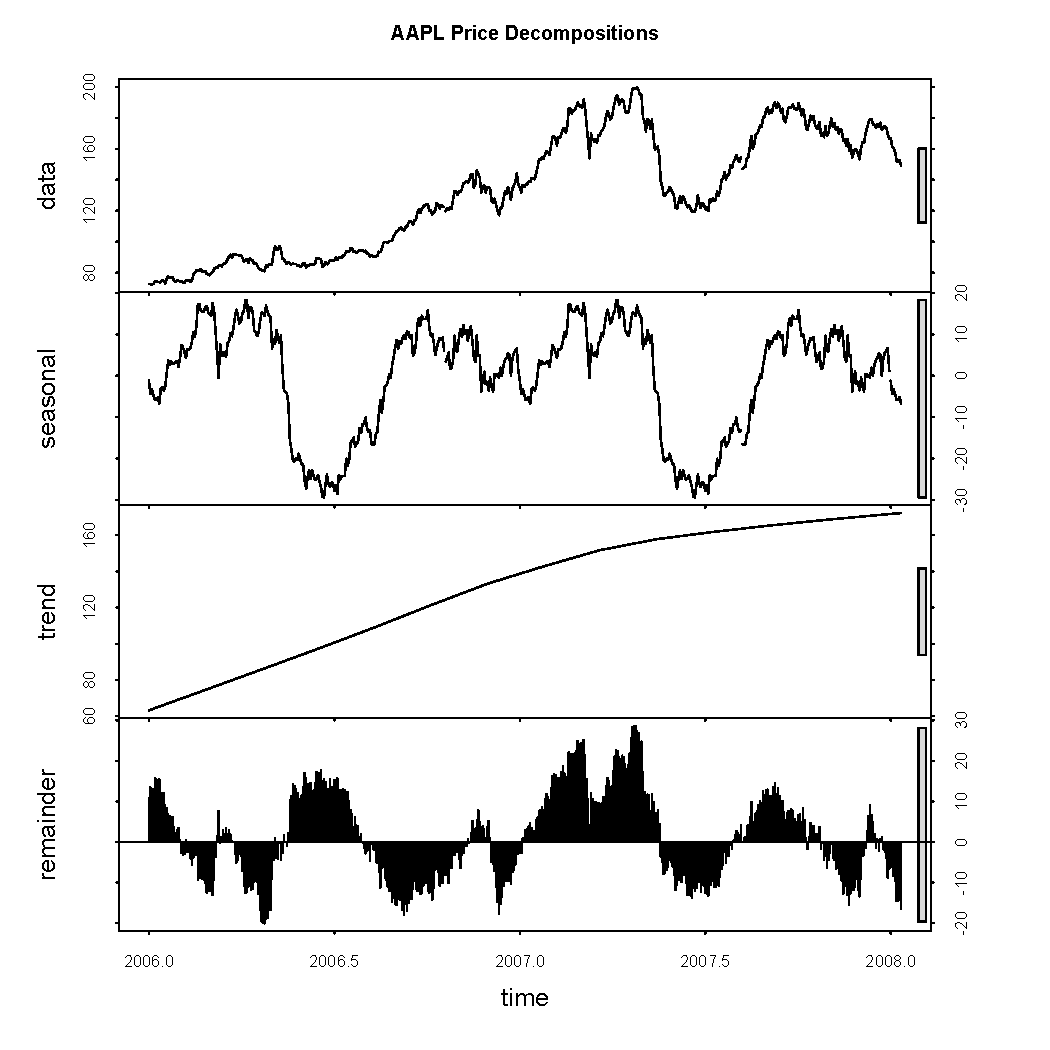
\includegraphics[scale=.7]{aapl-stl}
  \caption{AAPL Price Series Decomposition}
  \label{figure:aapl-stl}
\end{figure}

We can use R to create a decomposition of the AAPL time series, which displays the data, seasonal pattern, trend, and the remainder. The decomposition is displayed in Figure~\ref{figure:aapl-stl}. There are four factors that influence time series as seen in Table~\ref{tab:factors-ts}. The R code follows.
\ecaption{Time Series Decomposition in R}
\begin{verbatim}
aaplts<-ts(aapl$Close,start=c(2006,1),frequency=250)
decomp<-stl(aaplts,"periodic")
plot(decomp)
\end{verbatim}

\begin{table}[htbp]
	\centering
	\begin{tabular}{llll}
	\toprule
	Factor & Definition & Duration \\
	\hline
	Trend & Overall persistent long-term movement & Years \\
	Seasonal & Regular pattern of periodic fluctuations per year & Within 12 mo. \\
	& & (weekly, annually, \textit{etc.}) \\
	Cyclical &	Repeating up/down swings & Several (2--10) years \\
	Irregular &	 Erratic, random variation & Non-repeating \\
	\bottomrule
	\end{tabular}
	\caption{Factors Influencing Time Series}
	\label{tab:factors-ts}
\end{table}

\subsubsection{Seasonal Differencing with Dummy Variables}\label{perform-ts}
We will take data from the 2004 \emph{Economic Report of the President} which contain many variables, but we are only concerned with, \textit{i3} the 3-month T-bill rate, \textit{inf} the annual inflation rate, and \textit{def} the federal budget deficit as a percentage of GDP. We want to calculate $\beta$ values for the equation,
\begin{equation}
\widehat{i3_t} = \beta_0 + \beta_1 inf_t + \beta_2 def_t.
\label{eq:ts-regress}
\end{equation}

We load the MATLAB data file \texttt{econrep} which has a matrix named \texttt{intdef}. The remaining steps to get our $\beta$ values are required to perform matrix division.

\ecaption{Time Series Regression in MATLAB}
\begin{verbatim}
     load econrep
     i3=intdef(:,2);
     inf=intdef(:,3);
     def=intdef(:,6);
     A=[ones(size(inf)) inf def];
     x=A\i3
     
     x =
         1.7333
         0.6059
         0.5131
\end{verbatim}

which allows us to fill in constants for \eqref{eq:ts-regress},
\[
\widehat{i3_t} = 1.7333 + 0.6059 \times inf_t + 0.5131 \times def_t.
\]
Next, we want to determine the $r^2$ value of this regression equation. However, we want to obtain an \emph{adjusted} $r^2$,
\begin{equation}
r^2_{adj} = 1- \Big( (1-r^2)\frac{n-1}{n-k-1} \Big),
\label{eq:adj-rsquared}
\end{equation}
where $n$ is sample size, and $k$ is degrees of freedom in the regression. This allows us to compare regressions with different numbers of independent variables. Adjusting $r^2$ in \eqref{eq:adj-rsquared} allows us to account for the number of parameters used in the regression.

\begin{verbatim}
     yhat=x(1) + x(2).*inf + x(3).*def;
     sst=sum((i3-mean(i3)).^2);
     sse=sum((yhat-mean(i3)).^2);
     ssr=sum((yhat-i3).^2);
     r_squared=sse/sst;
     n=size(i3,1);
     k=size(x,1)-1;
     adj_r2=1-((1-r_squared).*(n-1)/(n-k-1))
\end{verbatim}

We see that our $r^2=0.6021$ and adjusted $r^2=0.5871$.

\paragraph{Dummy Variables.}\index{Binary Variable|see{Dummy Variable}}\index{Dummy Variable}\label{dummy-variable}
Binary variables are also known as \emph{dummy variables}. In order to include an observed qualitative factor, we need to pick a variable that indicates what is represented by the number 1. Choosing $female=1$ is more clear than $gender=1$, which tells us nothing about what the value of 1 represents. %We can add a qualitative factor to \eqref{eq:ts-regress} by adding a dummy variable, giving us
\paragraph{Ordinal Variables.}Some qualitative variables are \emph{ordinal}, that is, they measure a factor that has more than two values. If we want to use season of the year as an independent variable, we need four values (Winter, Spring, Summer, Fall). It makes little sense to assign $S=1$ to Winter, and $S=2$ to Spring because Spring does not represent any quantity that is double the value of Winter.  Instead, we may assign a variable for each season (Table~\ref{tab:ord-variable}), so that we have,
\[
\hat{y} = \beta_0 + \delta_1 S_1 + \delta_2 S_2 + \delta_3 S_3 +\delta_4 S_4 + \epsilon.
\]

\begin{table}[tbp]
	\centering
	\begin{tabular}{lc}
	\toprule
	Season & Variables \\
	\hline
	Winter & $\mathbf{S_1=1}; S_2 = 0; S_3 = 0; S_4 = 0$ \\
	Spring & $S_1=0; \mathbf{S_2 = 1}; S_3 = 0; S_4 = 0$ \\
	Summer & $S_1=0; S_2 = 0; \mathbf{S_3 = 1}; S_4 = 0$ \\
	Fall & $S_1=0; S_2 = 0; S_3 = 0; \mathbf{S_4 = 1}$ \\
	\bottomrule
	\end{tabular}
   \caption{Ordinal Variable Setting}
   \label{tab:ord-variable}
\end{table}

One value they can add to time series analysis is in the form of an \emph{event study}.\index{Event Study} The variable can indicate the period in which a specific event occurred. If we add a dummy variable to \eqref{eq:ts-regress} that indicates if Congress has enacted a certain law,
\[
\widehat{i3_t} = \beta_0 + \beta_1 inf_t + \beta_2 def_t + \beta_3 d_t,
\]
then, with that dummy variable $d_t$ we can observe the effect of the law by measuring the estimators with the variable and without it.

\paragraph{Index Numbers.}
To construct an event study, we must often work with an \emph{index number}\index{Index Number}.  The Consumer Price Index (CPI), ``is a measure of changes in prices for purchases made by urban consumers only'' \cite[p. 91]{rogers-1998}. Essentially, it is the price of a specific basket of consumer goods at a specific point in time. The Bureau of Labor Statistics\index{Bureau of Labor Statistics (BLS)} publishes a national number as well as several regions CPI numbers.

An index number such as the CPI-U\footnote{The U.S. Department of Labor publishes a monthly ``All Urban Consumers'' Consumer Price Index (CPI-U) based on U.S. city average of a basket of consumer goods. The CPI website is located at \\ \texttt{http://www.bls.gov/cpi/home.htm}} means nothing on its own; the August 2008 level is 219.086, and is -0.4 percent lower than in the previous month. However, its value comes from comparing it to a \emph{base period}\index{Base Period}  which has a \emph{base value}\index{Base Value}.  Our August 2008 CPI-U has a base period of 1982--1984, and a base value of 100. From this point, we can determine the change in price level for consumers over a span of time. Additionally, we can adjust \emph{nominal dollars} into \emph{real dollars} by factoring inflation as measured by CPI changes.

Having made any adjustments using index numbers to our time series data, we may use them in time series regressions without distorting their value.

\subsubsection{Trend and Seasonality}\index{Time Series!trend and seasonality}
Referring back to Figure~\ref{figure:aapl-stl}, we see that econometric models calculate the level, trend and seasonality and combine them to arrive at a forecast. It is not possible to understand the nature of trend and seasonality simply by viewing the data in the graphical screen. Decomposing time series data into trend and seasonality provides insights into the patterns of these components. This helps us choose the right forecast strategy or in setting the
parameters for a particular strategy.

Isolating the trend component requires neutralizing the seasonal effect in the data. If the data has a 12 period seasonality, computing a 12 period \emph{moving average} neutralizes the effect of seasonality. With a history of 24--36 months, we can calculate the trend for 13--25 months. Viewing the trend graphically provides insights into the way trend is changing over the analysis period. We can assess from this graph if the short term trend is in line with the long term trend. The short term trend is relevant for operational decisions like trading whereas the long term trend would be relevant for annual budgeting and other capital expenditure decisions.

Since the time series is a combination of trend, seasonality and randomness, subtracting the trend from the time series will leave us with seasonality and randomness. The seasonal patterns can be viewed graphically at different aggregate levels. If the time series has
seasonality, one will be viewing recurring patterns at periodic intervals. If there is no seasonality, there will not be any recurring patterns but only random patterns.

%\paragraph{Durbin-Watson Statistic.}\index{Durbin-Watson statistic}
%\subsection{Fractionally Differenced Models}\index{Fractionally Differenced Models}
%\subsection{Long-Memory Modeling}